\documentclass{beamer}


%\beamertemplateshadingbackground{yellow!100}{white}
\usepackage[english]{babel}
\usepackage{amsfonts,amsmath}
\usepackage{graphicx}
\usepackage{sansmathaccent}
\pdfmapfile{+sansmathaccent.map}
\usepackage{multirow}
%\usetheme{Warsaw}
\usetheme[secheader]{Madrid}

\usepackage{multimedia}
\logo{
\includegraphics[height=0.5cm]{imi.jpg}}

\newcommand{\be}{\begin{equation}}
\newcommand{\ee}{\end{equation}}
\newcommand{\rf}[1]{(\ref{#1})}
\newcommand{\RR}{\mathbb{R}}
\newtheorem{thm}{Theorem}
\newtheorem{lm}{Lemma}

%\def\ra#1\{\renewcommand{\arraystretch}{#1}
\begin{document}
 %[propagating wave solutions to the 2D BPE]
\title{Comparison between two numerical methods for solution of 2D Boussinesq paradigm equation}

%\author[K. Angelow]{{\underline{Krassimir Angelow}}, Natalia Kolkovska}
\author[K. Angelow]{{\underline{Krassimir Angelow}} }
\institute[IMI -- BAS]{Institute of Mathematics and Informatics\\ Bulgarian Academy of Sciences, Sofia, Bulgaria,\\ e-mail: angelow@math.bas.bg}
%\date[2021]{AMITANS, June 20-25  2021,  Albena, Bulgaria}
\date[2021]{May 27  2021,  Institute of Mathematics and Informatics, Bulgarian Academy of Sciences}


%---------- frame 01 ----------------
\begin{frame}
 \titlepage
 \begin{center}
  Supported by Bulgarian National Science Fund Grant K$\Pi$-06-H22/2
  \end{center}
\end{frame}

%---------- frame 02 ----------------
\begin{frame}
\tableofcontents 
\setbeamertemplate{table of contents shaded}[default]
\section{Boussinesq Paradigm Equation}
\section{Quadrature Formulas}
\section{Numerical Methods}
\subsection{Conservative Finite Difference Scheme (FDS) }
\subsection{Taylor Series (TS) Approach with Method of Lines }
%---------- frame 06 ----------------
\section{Convergence}

%---------- frame 07 ----------------
\section{Comparison Between TS and Conservative Scheme}
%\tableofcontents 
\end{frame}

%---------- frame 03 ----------------
\begin{frame}
\frametitle{Boussinesq Paradigm Equation}


The standard two dimensional BPE formulation is

\begin{align}\label{problem}
 \frac{\partial^2 u}{\partial t^2}= \Delta u + \beta_1 \Delta \frac{\partial^2}{\partial t^2} u -  \beta_2 \Delta^2 u +  \alpha \Delta (u^2)
\\
u(x,y,0) = u_0(x,y), \quad \frac{\partial u}{\partial t}(x,y,0)=u_1(x,y), \nonumber
\\
u(x,y,t) \rightarrow 0, \quad \Delta u(x,y, t) \rightarrow 0 \quad \text{for} \quad \sqrt{x^2+y^2} \rightarrow \infty \nonumber
\end{align}
where $\alpha>0$, $\beta_1>0$, $\beta_2>0$  are dispersion parameters, and $\Delta$ is the Laplace operator. The domain of the unknown function $u$ is defined by:
\be
 u:\Omega \times [0, T] \rightarrow R
\ee
where $\Omega \in R^2$ and $T>0$.
\end{frame}

%---------- frame 04 ----------------

\begin{frame}
\frametitle{Boussinesq Paradigm Equation}


The stationary two dimensional solitary wave is defined by
$$U(x, y-ct) = u(x, y, t)$$
and evaluated in 
\begin{description}
 \item[1] Christou, Christov, Galerkin Spectral Method for the 2D Solitary Waves of Boussinesq Paradigm Equation, 
 \item[2] Christou, Christov, Fourier-Galerkin Method for 2D Solitons of Boussinesq Equation, 
  \item[3] Christov, Choudhury, The Perturbation Solution for the 2D Boussinesq Equation,
  \item[4] K. Angelow, N. Kolkovska, Numerical Study of TWS to 2D Boussinesq Equation.
\end{description}

Remarks:
\begin{description}
 \item[-] [1] and [2] uses FDS with $O(h^2)$ approximation, 
  \item[-] [3] - the" best fit" formulas for small speeds $c$.
\end{description}
%Numerical Realization of Unsteady Solutions for the 2D Boussiensq Paradigm Equation, Christov, Kolkovska, Vasileva
% represents another methodology based on "best fit" formulas which is applicable for small speeds $c$.
% using two numerical methods with $O(|h|^2 + \tau^2)$ error is
\end{frame}

%---------- frame 05 ----------------

\begin{frame}
\frametitle{Boussinesq Paradigm Equation}


Based on the solutions of the stationary equation, the 2D hyperbolic equation is solved numerically in 
\begin{description}
 \item[5] Christov, Vasileva, Kolkovska, Numerical Realization of Unsteady Solutions for the 2D BPE,
 \item[6] Chertock, Christov, Kurganov, Central-Upwind Schemes for the Boussinesq Paradigm Equations, 
  \item[7] Angelow, Kolkovska, A Multicomponent Alternating Direction Method for Numerical Solving of Boussinesq Paradigm Equation,
\item[8] M. Dimova, D. Vasileva, Comparison of Two Numerical Approaches to Boussinesq Paradigm Equation.
\end{description}
\end{frame}

%---------- frame 06 ----------------

\begin{frame}
\frametitle{Boussinesq Paradigm Equation}

The goal of this talk is to:
\begin{itemize}
 \item propose numerical method with high order approximation for the solution of BPE,
 \item investigate properties of the resulting waves for velocities, which are close to the maximum $c \approx c_{max}$, $c < c_{max}$:
	\begin{itemize}
	 \item mass,
	 \item energy,
	 \item shape,
	 \item maximum,
	\end{itemize}
\end{itemize}
where $c_{max} = max(1, \sqrt{ \frac{\beta_2}{\beta_1} } )$.
\end{frame}


%---------- frame 07 ----------------

\begin{frame}
\frametitle{Boussinesq Paradigm Equation}
The following variable change
\begin{align}
x = \sqrt{\beta_1} \bar{x}, \quad y = \sqrt{\beta_1} \bar{y}, \quad t = \sqrt{\beta_1} \bar{t}
\end{align}

transforms (1) into 

\be\label{problemVC}
\beta(I-\Delta) \frac{\partial^2 u}{\partial t^2}=
  \Delta u -\Delta^2 u +\Delta(-\alpha \beta u^2 + (\beta - 1 )u)
\ee

where $\beta = \beta_1/\beta_2$.

\end{frame}



%---------- frame 05 ----------------
\begin{frame}
\frametitle{Conservation of the Mass and Energy}
The mass:

\begin{equation}\label{int}
D(u(t))=D(u(0))=\int_{R^2} u(x,y)dx dy
\end{equation}

and energy:
\begin{align}\label{ex-en}
E(u(t)) = E(u(0)) =&\int_{R^2} u_t \left((A^{-1}+E)u_t\right) dxdy+
\beta \int_{R^2} u^2 dxdy \nonumber\\
+& \int_{R^2}u \left(A u\right) dxdy
-\frac{2 \alpha \beta}{3} \int_{R^2} u^3 dxdy =const
\end{align}
of the continuous problem \rf{problem}. Here $E(u)$ is the exact energy of problem \rf{problem} and $Au=-\Delta u$.
\end{frame}

%-----------------------------------------------------------------

\begin{frame}
\frametitle{The Computational Domain $\Omega_h$}
\framesubtitle{Equidistant Grid $h=(h_1, h_2)$}
\begin{center}\vspace{0.4cm}
	\begin{minipage}[b]{0.6\linewidth}
		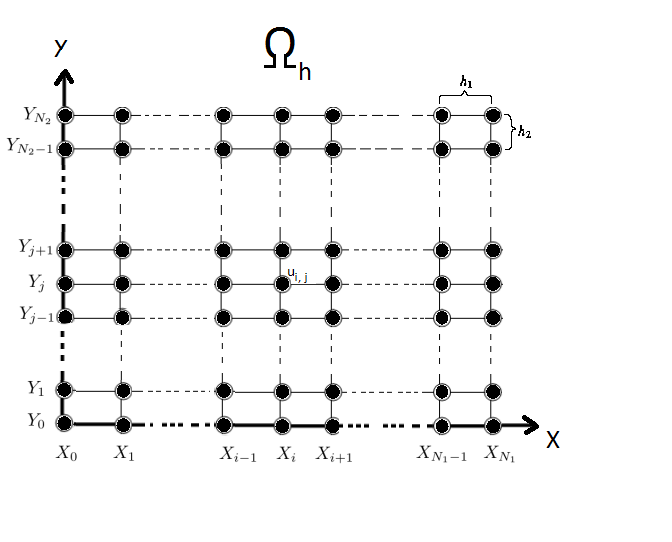
\includegraphics[width=\linewidth]{Omega_dah.png}
	\end{minipage}
\end{center}

\end{frame}

%---------- frame ----------------

\begin{frame}
\frametitle{Quadrature Formulas for the Mass and Energy}
\framesubtitle{\textbf{2D trapezoidal formula} (with global $O(h_1^2+h_2^2)$ error)}

Let's assign the X,Y dimensions of the computational domain with $N_1$ and $N_2$.
Then the approximation of the integral \eqref{int} with global $O(h_1^2+h_2^2)$ error is

\begin{align}\label{quadr2}
D_h(u_{i,j}) =& \sum_{i=1}^{N_1-1} \sum_{j=1}^{N_2-1} h_1 h_2 u_{i,j}
+\frac{h_1}{2}\sum_{i=0} \sum_{j=1}^{N_2-1} h_2 u_{i,j}
+\frac{h_1}{2}\sum_{i=N_1} \sum_{j=1}^{N_2-1} h_2 u_{i,j} \nonumber\\
+&\frac{h_2}{2}\sum_{j=0} \sum_{i=1}^{N_1-1} h_1 u_{i,j}
+\frac{h_2}{2}\sum_{j=N_2} \sum_{i=1}^{N_1-1} h_1 u_{i,j}
\nonumber\\
+&\frac{1}{4}h_1 h_2 \left(u_{0,0}+u_{N_1,0}+u_{N_1,N_2}+u_{0,N_2}
\right).
\end{align}

\end{frame}

\begin{frame}
\frametitle{Quadrature Formulas for the Mass and Energy}
\framesubtitle{\textbf{2D Simpson's rule} (with global $O(h_1^4+h_2^4)$ error)}
Assume that $N_1=2k$, $N_2=2 l$.
For every $m=0,1,2,\cdots N_2$ we compute 

$$D_m= \frac{h_1 }{3} 
\left\{ u_{0,m}+u_{N_1,m}+ 4 \sum_{i=1}^{\frac{N_1}{2}}   u_{2i-1,m}
 +2 \sum_{i=1}^{\frac{N_1}{2}-1} u_{2i,m} \right\}$$


Then 

\begin{equation}\label{quadr4}
D_h(u)=\frac{h_2 }{3} 
\left\{ D_{0}+D_{N_2}+ 4 \sum_{j=1}^{\frac{N_2}{2}}   D_{2j-1}
 +2 \sum_{j=1}^{{\frac{N_2}{2}}-1} D_{2j} \right\}
\end{equation}
is the approximation of the integral \eqref{int} with global $O(h_1^4+h_2^4)$ error

\end{frame}

%------------------------------------------------------------------

\begin{frame}
\frametitle{Quadrature Formulas for the Mass and Energy}
\framesubtitle{\textbf{2D Boole's rule} (with global $O(h_1^6+h_2^6)$ error)}

Assume that $N_1=4k$, $N_2=4 l$.
For every $m=0,1,2,\cdots N_2$ we compute

\begin{align*}
D_m =& \frac{2h_1}{45} 
\left\{
7u_{0,m}+7u_{N_1,m}+32 \sum_{i=1}^{\frac{N_1}{2}}u_{2i-1,m}
+12\sum_{i=1}^{\frac{N_1}{4}}u_{4i-2,m}
+14 \sum_{i=1}^{\frac{N_1}{4}-1}u_{4i,m}
\right\}
\end{align*}

then \eqref{quadr6-2D} is the approximation to the integral \eqref{int} with global $O(h_1^6+h_2^6)$ error

\begin{align}\label{quadr6-2D}
&D_h(u) =
\frac{2h_2}{45} 
\left\{
7D_{0}+7D_{N_2}+32 \sum_{j=1}^{\frac{N_2}{2}}D_{2j-1}
+12\sum_{j=1}^{\frac{N_2}{4}}D_{4j-2}
+14 \sum_{j=1}^{\frac{N_2}{4}-1}D_{4j}
\right\}
\end{align}
\end{frame}

%------------------------------------------------------------------

\begin{frame}
\frametitle{Conservative FDS}
The approximation of the differential operators is defined as:
\begin{equation}
\frac{\partial^2 u}{\partial t^2}(x_i, y_j, t_k ) = \frac{ u^{(k+1)}_{i, j} - 2u^{(k)}_{i,j} + u^{(k-1)}_{i,j} }{\tau^2} + O(\tau^2) 
\end{equation}

\begin{equation}
\frac{\partial^2 u}{\partial x^2}(x_i, y_j, t_k ) = \frac{ u^{(k)}_{i+1, j} - 2u^{(k)}_{i,j} + u^{(k)}_{i-1,j} }{h_1^2} + O(h_1^2) 
\end{equation}

\begin{equation}
\frac{\partial^2 u}{\partial y^2}(x_i, y_j, t_k ) = \frac{ u^{(k)}_{i, j+1} - 2u^{(k)}_{i,j} + u^{(k)}_{i,j-1} }{h_2^2} + O(h_2^2) 
\end{equation}


\begin{equation}
\Delta_h u(x_i, y_j, t_k )  = \frac{ u^{(k)}_{i+1, j} - 2u^{(k)}_{i,j} + u^{(k)}_{i-1,j} }{h_1^2} + \frac{ u^{(k)}_{i, j+1} - 2u^{(k)}_{i,j} + u^{(k)}_{i,j-1} }{h_2^2}
\end{equation}

\end{frame}

%------------------------------------------------------------------

\begin{frame}
\frametitle{Conservative FDS}
The grid function obtained from [\ref{problemVC}] is defined as:
\begin{equation}
\beta (I-\Delta_h)\frac{ u^{(k+1)}_{i, j} - 2u^{(k)}_{i,j} + u^{(k-1)}_{i,j} }{\tau^2} = (\Delta_h - \Delta_h^2)u^{(k)}_{i,j} + \Delta_h(g(u^{(k)}_{i,j}))
\end{equation}
%
where the non-linear term $g$ is defined as:
\begin{align}
g(u^{(k)}_{i,j})=& -\frac{\alpha \beta} { 3 } \left( (u^{(k+1)}_{i,j})^2 + (u^{(k-1)}_{i,j})(u^{(k+1)}_{i,j}) + (u^{(k-1)}_{i,j})^2 \right) + \nonumber\\
+&\frac{ (\beta - 1 )}{ 2 }\left( u^{(k+1)}_{i,j} + u^{(k-1)}_{i,j} \right).
\end{align}


\end{frame}


%------------------------------------------------------------------

\begin{frame}
\frametitle{TS Approach with Method of Lines}
\begin{center}\vspace{0.25cm}
	\begin{minipage}[b]{0.45\linewidth}
		 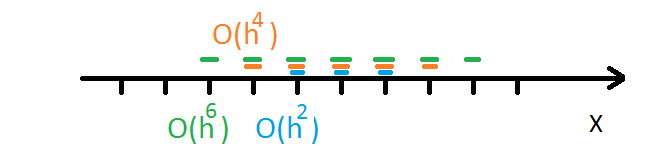
\includegraphics[width=\linewidth]{figures/FDS.png}
	\end{minipage}	
\end{center}
Let $\Delta_h u_{i,j}$ be the approximation of $\Delta u$ with $O(|h|^2)$, $O(|h|^4)$, $O(|h|^6)$.
\\
Let $u_{i,j}(t)$ be the approximation of $u(x_i, y_j, t)$ at grid point $(x_i, y_j)$.
\\
%here99
From [\ref{problemVC}] one obtains a system of ODEs:
\be \label{DiscreteEq}
\beta (I-\Delta_h) \frac{\partial^2 u}{\partial t^2}(x_i, y_j, t)=
 (\Delta_h - \Delta_h^2) u_{i, j}(t) + \Delta_h ( g( u_{i, j}(t) ) )
\ee
for $i = 0..N_1$ and $j=0..N_2$. For each ODE in the system we do TS expansion:
\begin{align} \label{TSe}
u(x_i, y_j, t+\tau) = u(x_i, y_j, t) + \tau \frac{ \partial u }{ \partial t }(x_i, y_j, t)  + ... 
%\nonumber
%\\
\frac{ \tau^p }{ p! } \frac{ \partial^p u }{ \partial t^p }(x_i, y_j, t) + O(\tau^{p+1})
\end{align}
for some natural number $p \ge 2$.
%Suppose we have functions $y$ and $f$ with the following properties
%\begin{equation}
%y:I \rightarrow \RR, \quad f:I \times \Omega \rightarrow \RR \nonumber
%\end{equation}
%where $y \in C^1(I,\RR)$ and $f$ is sufficiently smooth on $I \times \Omega$. Then, $f$ represent the phase space and $y$ is the unknown function to the differential equaiton:
%\begin{equation}
%\dot{y}(t) = f(t, y(t)).
%\end{equation}
%By repeated differentiation we can find each function

%\begin{equation}
%\frac{d^s}{dt^s}y(t) = \frac{d^{s-1}}{dt^{s-1}}f(t, y(t))
%\end{equation}

%and evaluate it at $t=t_0$ for each derivative.
\end{frame}

%------------------------------------------------------------------

\begin{frame}
\frametitle{TS Approach with Method of Lines}
Evaluating formula [\ref{TSe}]
\begin{itemize}
 \item IC $\rightarrow$ $u(x_i, y_j, t=0)$, $\frac{ \partial u }{ \partial t }(x_i, y_j, t=0)$,
 \item $[$\ref{DiscreteEq}$]$ $\rightarrow$ $\frac{ \partial^2 u }{ \partial t^2 }(x_i, y_j, t=0)$ ,
 \item Differentiating equation $\frac{ \partial^{p-2} u }{ \partial t^{p-2} }$ [\ref{DiscreteEq}] $\rightarrow$  $\frac{ \partial^p u }{ \partial t^p }(x_i, y_j, t)$,
 \item Substitute the evaluated derivatives in formula $[$ \ref{TSe} $]$.
\end{itemize}


Thus one gets the following approximations
\begin{description}
 \item[$p=2$] $O(|h|^2 + \tau^2)$,
 \item[$p=4$] $O(|h|^4 + \tau^4)$,
 \item[$p=6$] $O(|h|^6 + \tau^6)$.
\end{description}

\end{frame}

%------------------------------------------------------------------

\begin{frame}
\frametitle{Validation and Results}
Two parameters sets are used:
\begin{description}
 \item[Test 1] $\beta = 3$, $c = 0.45$, $\Omega = [-30, 30] \times [-27, 27]$
 \item[Test 2] $\beta = 1$, $c = 0.9$, $\Omega = [-128, 128] \times [-58, 58]$
\end{description}

The tests use zero boundary condition, i.e. values of the finite difference stencil outside the numerical domain $\Omega_h$ are zeros.
\end{frame}


%------------------------------------------------------------------

\begin{frame}
\frametitle{Validation and Results}
\framesubtitle{The Wave}

\begin{center}\vspace{0.4cm}
	\begin{minipage}[b]{0.45\linewidth}
		 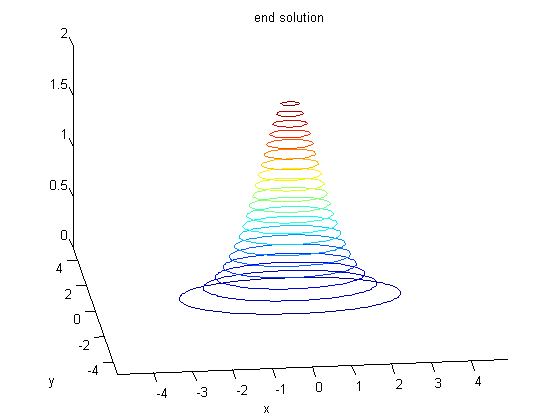
\includegraphics[width=\linewidth]{figures/nivoLines_bt3.png}
	\end{minipage}	
	\begin{minipage}[b]{0.45\linewidth}
		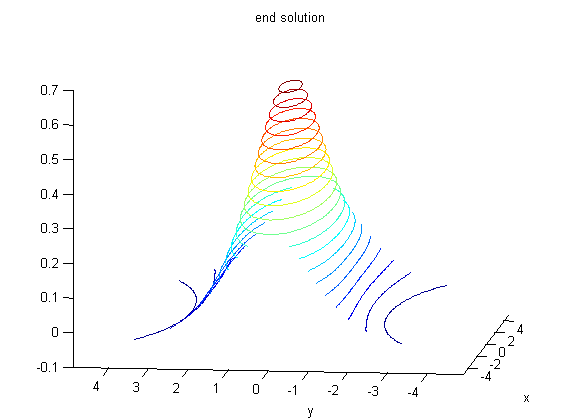
\includegraphics[width=\linewidth]{figures/nivoLines_bt1.png}
		
	\end{minipage}

\end{center}
The wave at $T=0$ for Test 1 (left) and Test 2 (right) localized in $[-5,5]\times[-5,5]$.

\end{frame}

%------------------------------------------------------------------

\begin{frame}
\frametitle{Convergence for TS Approach}
%A
$T = 10$
\begin{table}[ht]
\centering
\small
\resizebox{0.6\linewidth}{!}{%
		\begin{tabular}{||c|l|ll|ll||}
			\hline
			\hline
      \multirow{2  }{*}{FDS}        & \multirow{2  }{*}{$h$, $\tau$}  & \multirow{2  }{*}{errors $E_i$in$L_2$}  &Conv.& \multirow{2  }{*}{errors $E_i$in$L_\infty$}  &Conv.  \\
	         &                    &                               & Rate   &                                        & Rate \\
   			\hline 
					\hline 
  $\beta=3$                &0.2, 0.001          &              &              &                     &      \\
   c=0.45                     &0.1, 0.0005          &0.989414 &            &1.043641    &       \\
     $O(h^2 + \tau^ 2)$ &0.05, 0.00025   & 0.344813 & 1.52    &0.355511    &  1.55      \\
			\hline 
  $\beta=3$               &0.2, 0.02       &              &            &                     &      \\
   c=0.45                    &0.1, 0.01      &0.191224 &            &0.193874    &       \\
     $O(h^4+ \tau^4)$ &0.05, 0.005&0.013029 & 3.87   &0.013656     &3.82       \\
			\hline 
  $\beta=3$               &0.2, 0.02       &                &            &                     &      \\
     c=0.45                 &0.1, 0.01        &0.032671 &            &  0.033626    &       \\
     $O(h^6+ \tau^6)$ &0.05, 0.005 &0.000598 &5.77     & 0.000635    & 5.72       \\
	   \hline
			\hline 
       $\beta=1$       &0.4, 0.002        &             &            &           &   \\
                  c=0.9    &0.2, 0.001       &  0.20366   &            &0.075854 &   \\
  $O(h^2+ \tau^2)$ &0.1, 0.0005   &0.048320   &2.07  &0.022307  & 1.77 \\
			\hline
      $\beta=1$               &0.4, 0.04    &            &               &             &    \\
       c=0.9                     &0.2, 0.02     & 0.028275   &        &  0.013518   &   \\
       $O(h^4+ \tau^4)$ &0.1, 0.01   &0.001812 & 3.96  & 0.000971  & 3.80  \\
    \hline
  $\beta=1$     &0.4, 0.04   &            &          &                  &      \\
      c=0.9                    &0.2, 0.02   &0.006734 &           & 0.003338      &       \\
     $O(h^6+ \tau^6)$ &0.1, 0.01 & 0.000232 &4.86 & 0.000069  & 5.60        \\
	   \hline
			\hline 
		\end{tabular}
		}%
		\caption{Convergence tests for Taylor method with zero boundary and different approximation errors $O(h^{2} + \tau^2 )$, $O(h^{4} + \tau^4 )$ and $O(h^{6} + \tau^6 )$. Errors $E_i$ are measured in $L_2$ and $L_\infty$ norms}
\label{table:A}
\end{table}

\end{frame}
%------------------------------------------------------------------

\begin{frame}
%C
\frametitle{Convergence for Conservative FDS}
$T = 10$
\begin{table}[ht]
\centering
\small
		\begin{tabular}{||c|l|ll|ll||}
			\hline
			\hline
      \multirow{2  }{*}{FDS}        & \multirow{2  }{*}{$h$, $\tau$}  & \multirow{2  }{*}{errors $E_i$in$L_2$}  &Conv.& \multirow{2  }{*}{errors $E_i$in$L_\infty$}  &Conv.  \\
	                                        &                                                     &                                                                 &  Rate &                                                                       & Rate \\
   			\hline 
					\hline 
  $\beta=3$                &0.2, 0.001         &                    &                &                  &                   \\
   c=0.45                     &0.1, 0.0005         & 0.989422   &                & 1.043649  &                   \\
     $O(h^2 + \tau^ 2)$ &0.05, 0.00025  &0.344818    & 1.52       & 0.355517   &   1.55   \\
	   \hline
			\hline 
       $\beta=1$           & 0.4, 0.002       &                   &           &                 &   \\
                  c=0.9       & 0.2, 0.001        & 0.200424   &          &0.072726  &   \\
  $O(h^2+ \tau^2)$  & 0.1, 0.0005       & 0.047899   & 2.06  &0.021451  & 1.76 \\
	   \hline
			\hline 
		\end{tabular}
		\caption{Convergence tests for the Conservative FDS method with zero boundary and approximation errors $O(h^{2} + \tau^2 )$. Errors $E_i$ are measured in $L_2$ and $L_\infty$ norms}
\label{tableC}
\end{table}

\end{frame}

\begin{frame}
\frametitle{Results}
\framesubtitle{Mass and Energy for the Conservative scheme and TS method}

\begin{center}\vspace{0.4cm}
	\begin{minipage}[b]{0.49\linewidth}
		 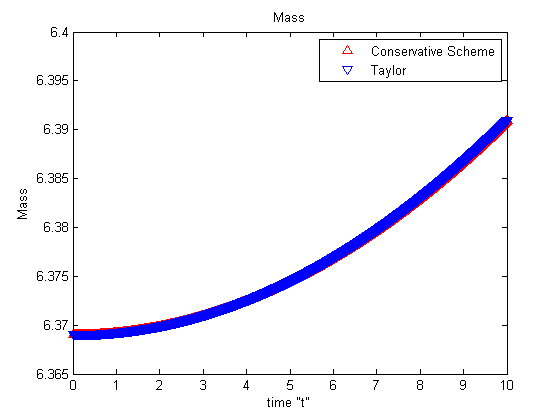
\includegraphics[width=\linewidth]{figures/Mass_bt3_c045_h005.png}
	\end{minipage}	
	\begin{minipage}[b]{0.49\linewidth}
		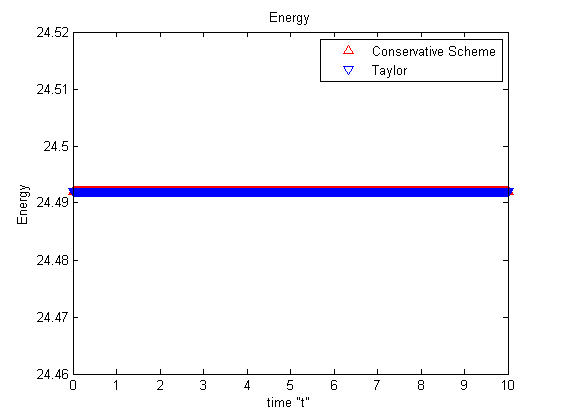
\includegraphics[width=\linewidth]{figures/Energy_bt3_c045_h005.png}
		
	\end{minipage}
\end{center}
The Mass (left) and Energy (right) of the solution for $\beta=3$, $c = 0.45$, $O(|h|^2 + \tau^2)$ and $T = 10$.
\end{frame}


\begin{frame}
\frametitle{Results}
\framesubtitle{Mass and Energy for the Conservative scheme and TS method}
%\framesubtitle{}

\begin{center}\vspace{0.4cm}
	\begin{minipage}[b]{0.49\linewidth}
		 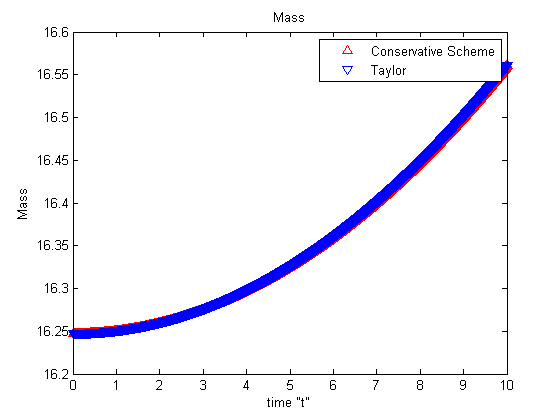
\includegraphics[width=\linewidth]{figures/Mass_bt1_c090_h010.png}
	\end{minipage}	
	\begin{minipage}[b]{0.49\linewidth}
		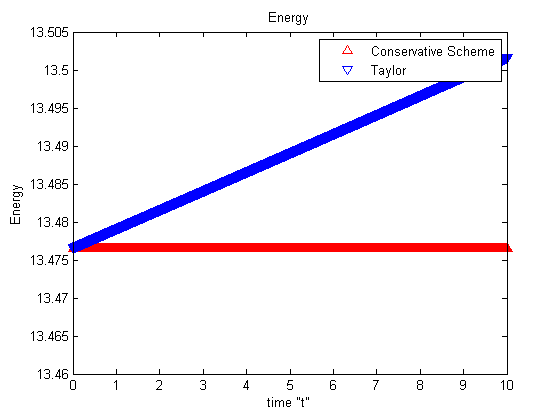
\includegraphics[width=\linewidth]{figures/Energy_bt1_c090_h010.png}
		
	\end{minipage}

\end{center}
The Mass (left) and Energy (right) of the solution for $\beta=1$, $c = 0.9$, $O(|h|^2 + \tau^2)$ and $T = 10$.
\end{frame}

%------------------------------------------------------------------

\begin{frame}
\frametitle{Results}
\framesubtitle{Mass and Energy for the TS method only}
%\framesubtitle{}

\begin{center}\vspace{0.4cm}
	\begin{minipage}[b]{0.49\linewidth}
		 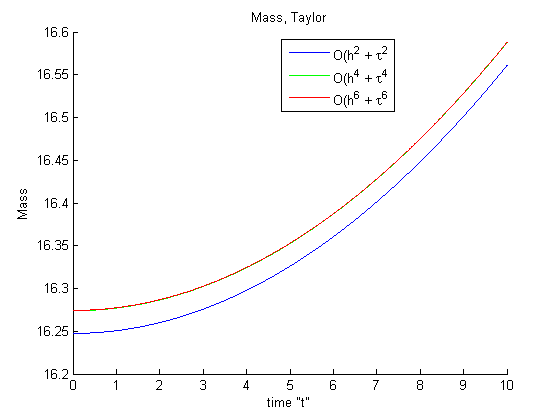
\includegraphics[width=\linewidth]{figures/Mass_bt1_c090_h010_x3O.png}
	\end{minipage}	
	\begin{minipage}[b]{0.49\linewidth}
		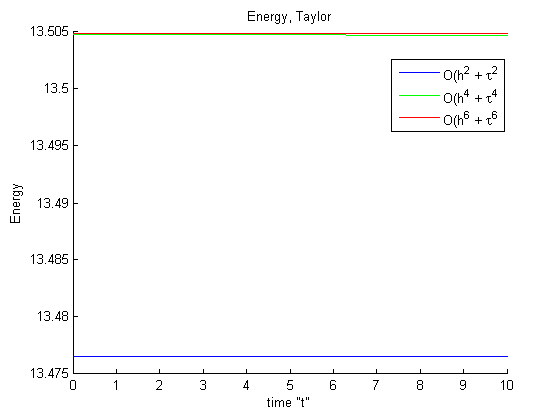
\includegraphics[width=\linewidth]{figures/Energy_bt1_c090_h010_x3O.png}
		
	\end{minipage}

\end{center}
The Mass (left) and Energy (right) of the Taylor solution for $\beta=3$, $c = 0.45$, $O(|h|^2 + \tau^2)$, $O(|h|^4 + \tau^4)$, $O(|h|^6 + \tau^6)$ and $T = 10$.
\end{frame}

%------------------------------------------------------------------


\begin{frame}
\frametitle{Results}
\framesubtitle{Mass and Energy for the TS method only}
%\framesubtitle{}

\begin{center}\vspace{0.4cm}
	\begin{minipage}[b]{0.49\linewidth}
		 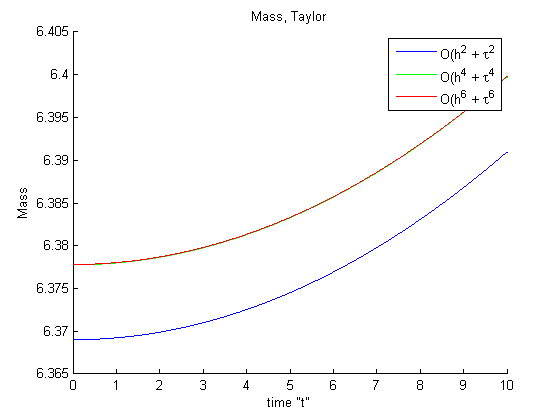
\includegraphics[width=\linewidth]{figures/Mass_bt3_c045_h005_x3O.png}
	\end{minipage}	
	\begin{minipage}[b]{0.49\linewidth}
		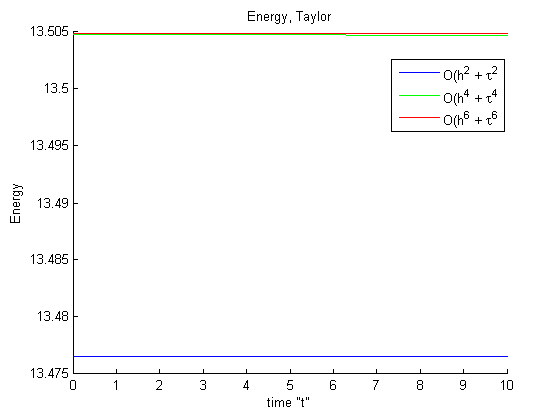
\includegraphics[width=\linewidth]{figures/Energy_bt1_c090_h010_x3O.png}
		
	\end{minipage}

\end{center}
The Mass (left) and Energy (right) of the Taylor solution for $\beta=1$, $c = 0.9$, $O(|h|^2 + \tau^2)$, $O(|h|^4 + \tau^4)$, $O(|h|^6 + \tau^6)$ and $T = 10$.
\end{frame}

%------------------------------------------------------------------



\begin{frame}
\frametitle{Results}
\framesubtitle{Wave Comparison}
\begin{center}\vspace{0.4cm}
	\begin{minipage}[b]{0.32\linewidth}
		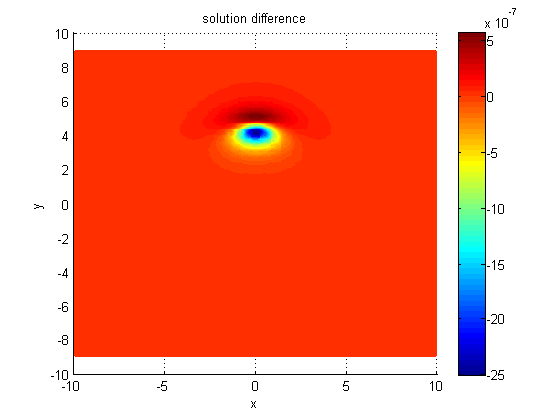
\includegraphics[width=\linewidth]{figures/compare_30_bt3_c045_h005.png}
	\end{minipage}	
	\begin{minipage}[b]{0.32\linewidth}
		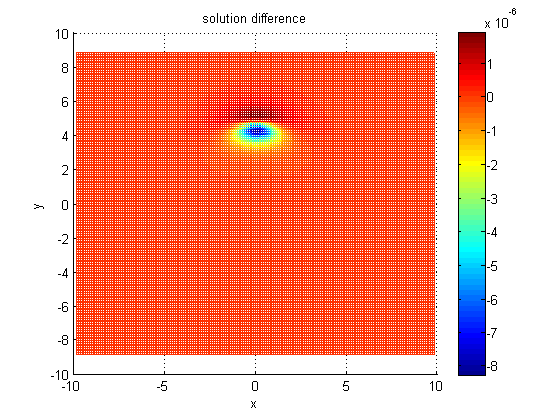
\includegraphics[width=\linewidth]{figures/compare_30_bt3_c045_h010.png}
	\end{minipage}	
	\begin{minipage}[b]{0.32\linewidth}
		 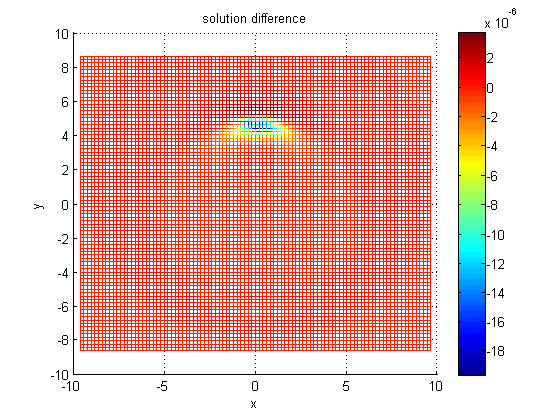
\includegraphics[width=\linewidth]{figures/compare_30_bt3_c045_h020.png}
	\end{minipage}
\end{center}
Difference between TS approach and Conservative Scheme at time $T=10$  for $\beta=3$, $c = 0.45$  and $O(|h|^2 + \tau^2)$. From Left to right $h=0.05, 0.1, 0.2$. The graphics represent only one nineth of the whole domain $\Omega_h$.
\end{frame}

%------------------------------------------------------------------

\begin{frame}
\frametitle{Results}
\framesubtitle{Wave Comparison}
\begin{center}\vspace{0.4cm}
	\begin{minipage}[b]{0.32\linewidth}
		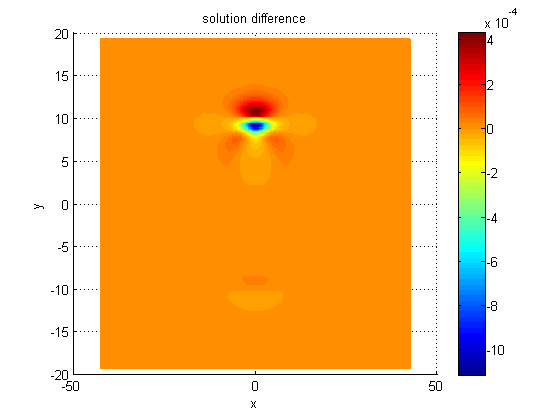
\includegraphics[width=\linewidth]{figures/compare_128_bt1_c09_h010.png}
	\end{minipage}	
	\begin{minipage}[b]{0.32\linewidth}
		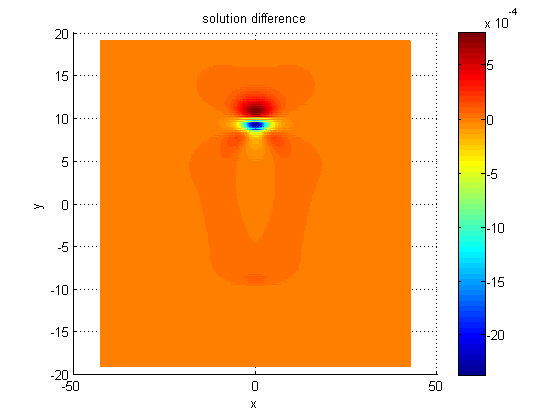
\includegraphics[width=\linewidth]{figures/compare_128_bt1_c09_h020.png}
	\end{minipage}	
	\begin{minipage}[b]{0.32\linewidth}
		 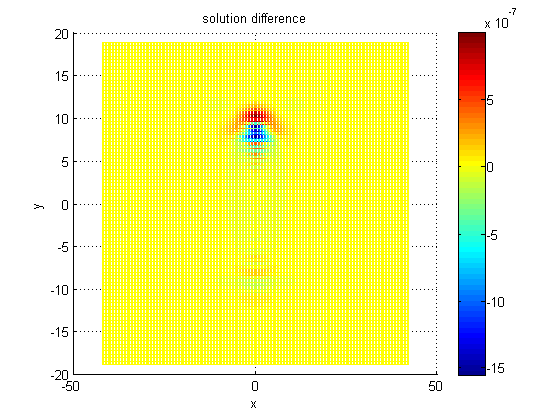
\includegraphics[width=\linewidth]{figures/compare_128_bt1_c09_h040.png}
	\end{minipage}
\end{center}
Difference between TS approach and Conservative Scheme at time $T=10$  for $\beta=1$, $c = 0.9$  and $O(|h|^2 + \tau^2)$. From Left to right $h=0.1, 0.2, 0.4$. The graphics represent only one nineth of the whole domain $\Omega_h$.
\end{frame}

%------------------------------------------------------------------

\begin{frame}
\frametitle{Results}
\framesubtitle{Solution Maximum}

Two parameters sets are used:
\begin{description}
 \item[Test 3] $\beta = 3$, $c = 0.52$, $\Omega = [-40, 40] \times [-40, 60]$
 \item[Test 4] $\beta = 1$, $c = 0.9$, $\Omega = [-40, 40] \times [-40, 80]$
\end{description}
The end time is $T=40$ for both tests.
\begin{figure}[ht]
	\centering
	\begin{minipage}[b]{0.4\linewidth}
		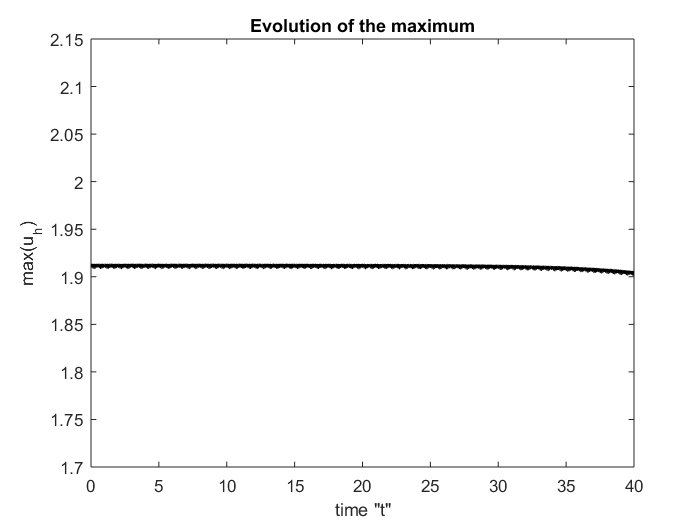
\includegraphics[width=\linewidth]{figures/EvolutionOfMaximum_bt3_t40.png}
	\end{minipage}	
	\begin{minipage}[b]{0.4\linewidth}
		 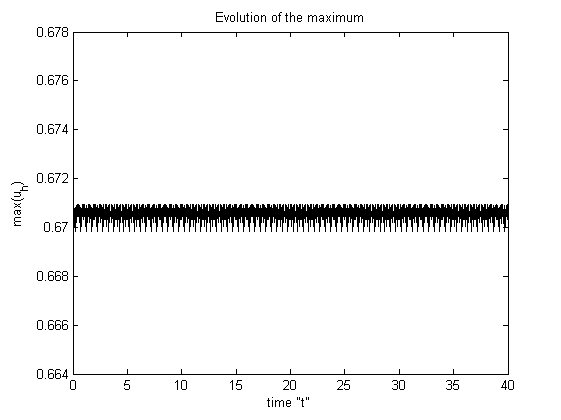
\includegraphics[width=\linewidth]{figures/EvolutionOfMaximum_bt1_t40.png}
	\end{minipage}

Evolution of the maximum for Test Wave $\beta =3$ (left panel) and $\beta=1$ (right panel).
\end{figure}

\end{frame}

%------------------------------------------------------------------

\begin{frame}
\frametitle{Results}
\framesubtitle{Wave Evolution}
\begin{center}\vspace{0.4cm}
	\begin{minipage}[b]{0.30\linewidth}
		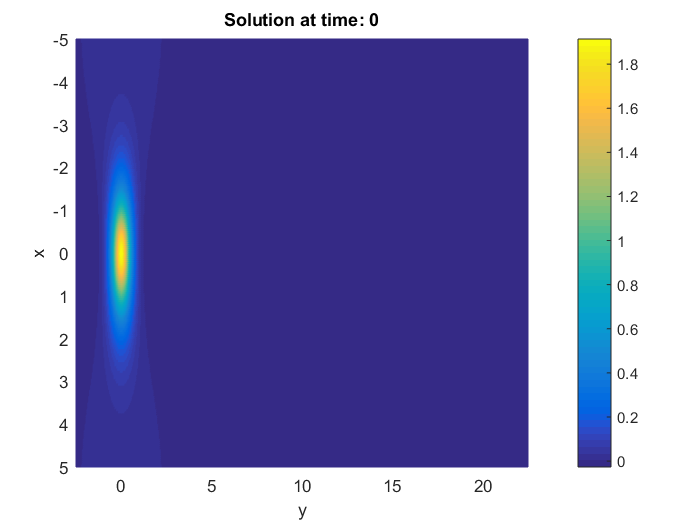
\includegraphics[width=\linewidth]{figures/Solution_bt3_t=0.png}
	\end{minipage}	
	\begin{minipage}[b]{0.30\linewidth}
		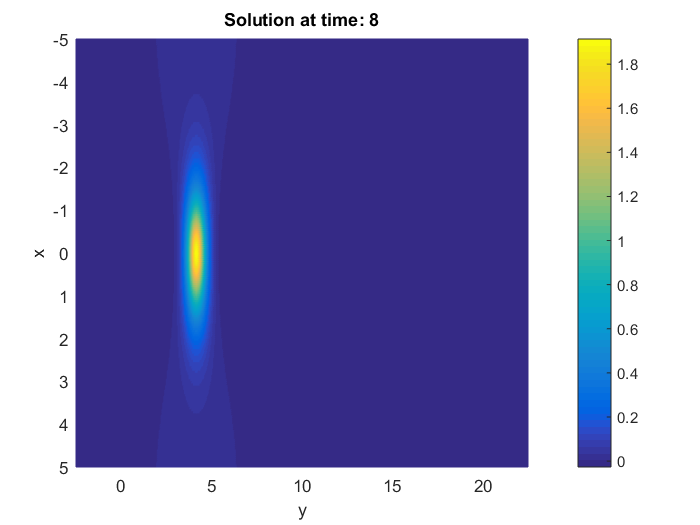
\includegraphics[width=\linewidth]{figures/Solution_bt3_t=8.png}
	\end{minipage}	
	\begin{minipage}[b]{0.30\linewidth}
		 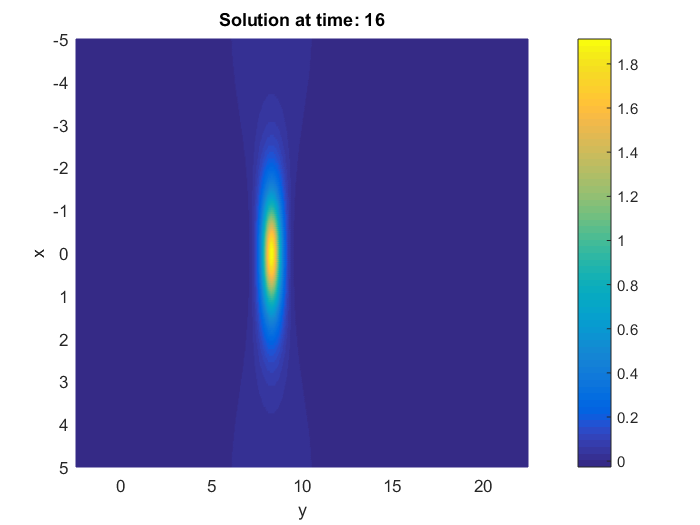
\includegraphics[width=\linewidth]{figures/Solution_bt3_t=16.png}
	\end{minipage}
	\begin{minipage}[b]{0.30\linewidth}
		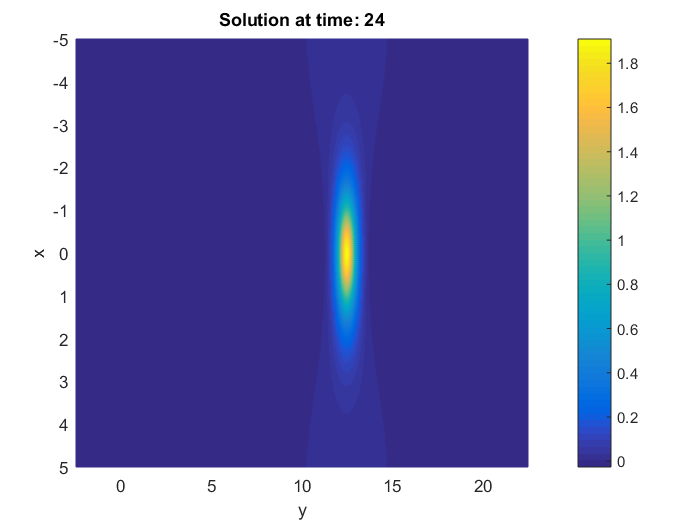
\includegraphics[width=\linewidth]{figures/Solution_bt3_t=24.png}
	\end{minipage}	
	\begin{minipage}[b]{0.30\linewidth}
		 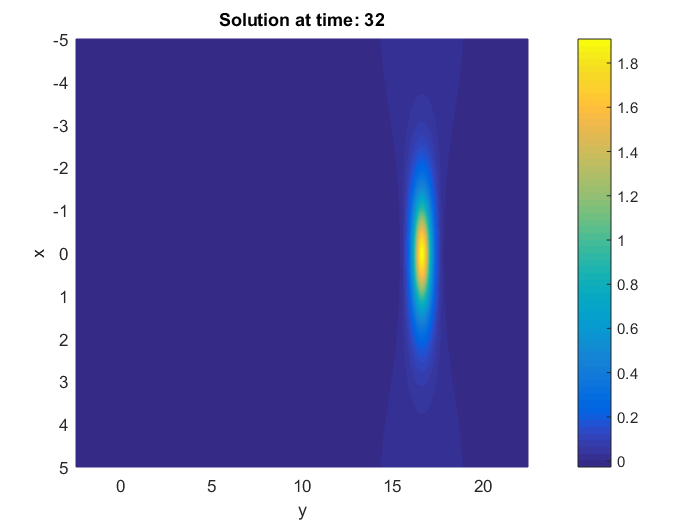
\includegraphics[width=\linewidth]{figures/Solution_bt3_t=32.png}
	\end{minipage}
	\begin{minipage}[b]{0.30\linewidth}
		 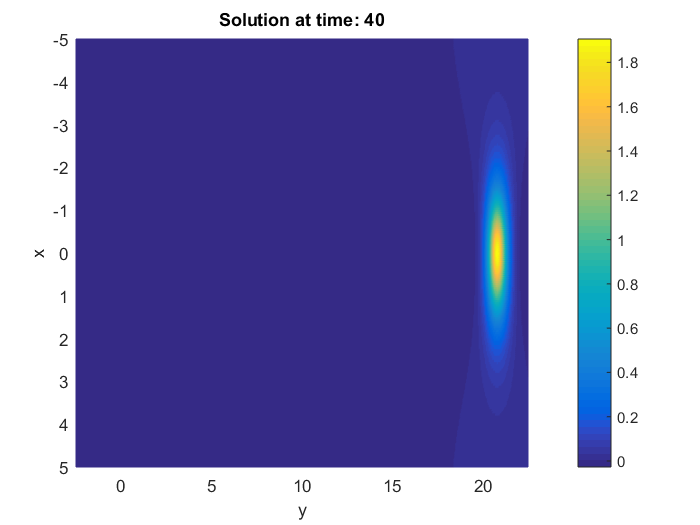
\includegraphics[width=\linewidth]{figures/Solution_bt3_t=40.png}
	\end{minipage}
\end{center}
Numerical solution of single wave for $\beta=3$ and $c = 0.52$ at times $t=0,8,16,24,32,40$.
\end{frame}

%------------------------------------------------------------------

\begin{frame}
\frametitle{Results}
\framesubtitle{Wave Evolution}
\begin{center}\vspace{0.4cm}
	\begin{minipage}[b]{0.30\linewidth}
		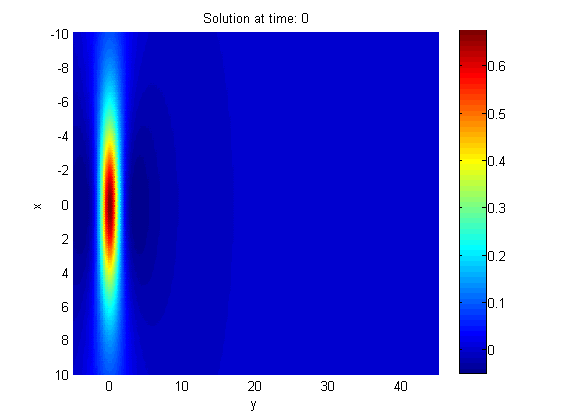
\includegraphics[width=\linewidth]{figures/Solution1_t=0.png}
	\end{minipage}	
	\begin{minipage}[b]{0.30\linewidth}
		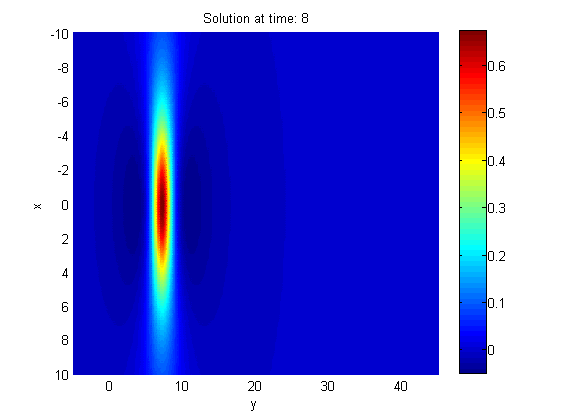
\includegraphics[width=\linewidth]{figures/Solution1_t=8.png}
	\end{minipage}	
	\begin{minipage}[b]{0.30\linewidth}
		 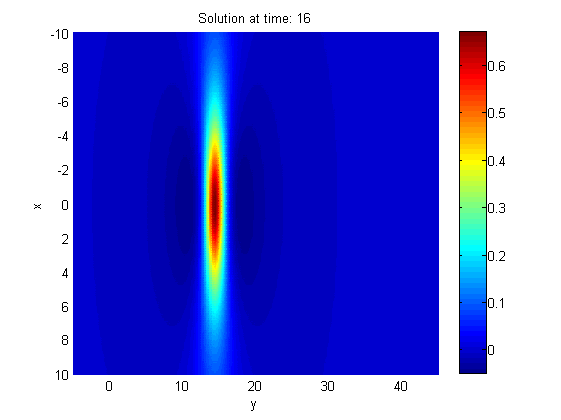
\includegraphics[width=\linewidth]{figures/Solution1_t=16.png}
	\end{minipage}
	\begin{minipage}[b]{0.30\linewidth}
		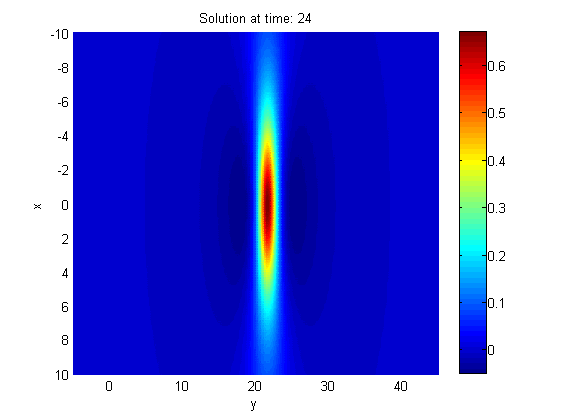
\includegraphics[width=\linewidth]{figures/Solution1_t=24.png}
	\end{minipage}	
	\begin{minipage}[b]{0.30\linewidth}
		 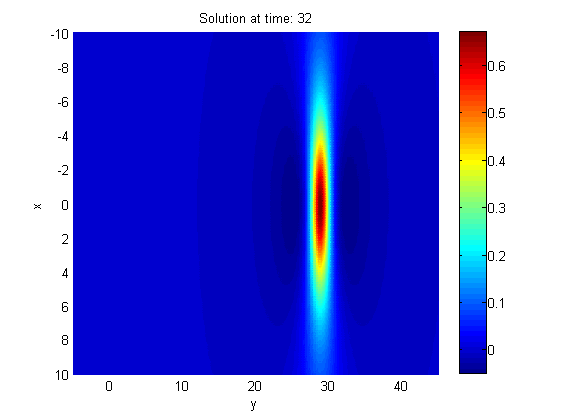
\includegraphics[width=\linewidth]{figures/Solution1_t=32.png}
	\end{minipage}
	\begin{minipage}[b]{0.30\linewidth}
		 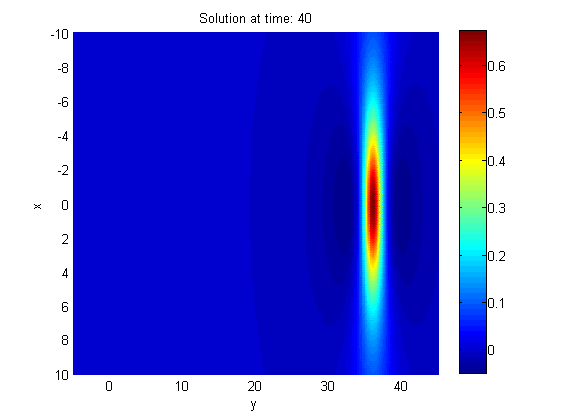
\includegraphics[width=\linewidth]{figures/Solution1_t=40.png}
	\end{minipage}
\end{center}
Numerical solution of single wave for $\beta=1$ and $c = 0.9$ at times $t=0,8,16,24,32,40$.
\end{frame}

%------------------------------------------------------------------

\begin{frame}
\frametitle{Results}
\framesubtitle{Solution Maximum}
\begin{figure}[ht]
	\centering
	\begin{minipage}[b]{0.49\linewidth}
		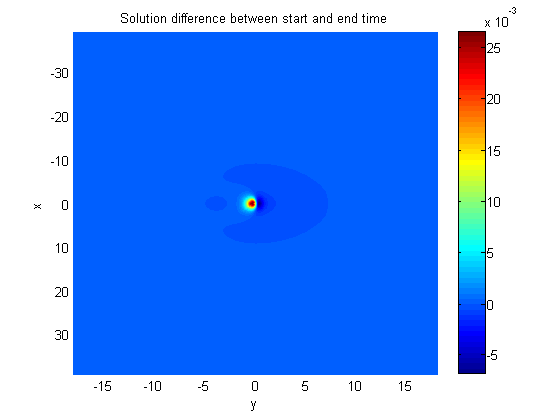
\includegraphics[width=\linewidth]{figures/compare_start_end_bt3_c052.png}
	\end{minipage}	
	\begin{minipage}[b]{0.49\linewidth}
		 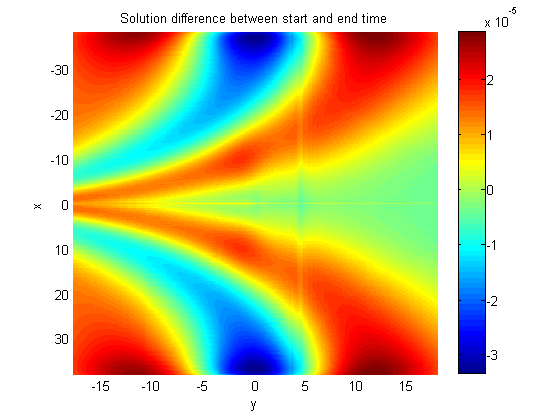
\includegraphics[width=\linewidth]{figures/compare_start_end_bt1_c09.png}
	\end{minipage}

Difference between localized solitons at time $T=0$ and $T=40$ for Test 3 $\beta = 3$, $\beta = 0.52$  (left) and Test 4 $\beta=1$, $c=0.9$ (right). 
\end{figure}

It is obtained that:
\begin{description}
 \item[$\beta = 3$, $c = 0.52$] $||u_h(t=40)-u_h(t=0)|_{L_2} = 0.023453$
 \item[$\beta = 1$, $c = 0.9$] $||u_h(t=40)-u_h(t=0)|_{L_2} = 0.000812$
\end{description}
\end{frame}

%------------------------------------------------------------------

\begin{frame}
\frametitle{Conclusion}

\begin{description}
 \item[-] 2D BPE is solved using TS method with high approximation orders $O(|h|^k+\tau^k)$, $k=2,4,6$
 \item[-] the results are compared with a Conservative Scheme for $O(|h|^2+\tau^2)$
 \item[-] the Energy and Mass of the TS solution are saved with high accuracy over the time interval $[0, 10]$
 \item[-] the resulting numerical solutions for wave speeds near the upper limit $c_{max} = min(1, \sqrt{\beta_2/\beta_1}$ are stable in form and their maximums are changed with small errors over long period of time $[0, 40]$.
\item[-] the obtained solutions show soliton behavior!
\end{description}

\end{frame}


\end{document}

